\section{Les CNN}

\fancyhead[R]{\textit{\nouppercase{\leftmark}}}

\subsection{Le modèle du CNN}

Bien qu'étant un modèle efficace, le perceptron reste coûteux en calcul : il faut réaliser les opérations matricielles sur tous les neurones de chaque couche.
Les réseaux neuronaux convolutifs (en anglais Convolutional Neural Network, CNN) permettent de réduire le nombre de calculs réalisés. Ils se basent sur la structure des données à classifier.
Les images sont un bon exemple de structure permettant de diminuer le nombre de calculs à réaliser. En effet, une image peut être caractérisée par les motifs locaux qui la constituent. Ces motifs sont en général localisés. Il n'est donc pas nécessaire de chercher un lien entre deux points éloignés d'une image.

Les CNN sont entraînés à chercher des motifs sur une partie restreinte de l'image.
Le principe est le même que celui des perceptrons, sauf qu'au lieu d'appliquer un réseau entièrement connectés sur toutes les couches, on va réaliser une convolution par différents filtres sur l'image. Chaque filtre aura pour but de détecter un motif dans l'image.

Une couche d'un CNN est typiquement constituée de 3 éléments : 

1) Une couche de convolution

2) Une couche d'activation 

3) Une couche de pooling


La couche de convolution prend en entrée une image de dimension (H, L, N) avec H la hauteur de l'image, L sa largeur et N le nombre de channels (pour une image RGB, on aura N = 3). 
On applique en parallèle sur cette image M filtres qui donneront M images de dimension deux. Ces filtres sont de même dimension (h, l, n) avec $h<H$, $l<N$ et $n=N$. On obtient donc M images de même dimension en sortie. Ces M images peuvent être vues comme une image à trois dimensions avec M channels. On peut alors répété le processus en considérant cette nouvelle image comme une entrée pour les M' filtres suivants.

\begin{figure}[h]
 \centering
 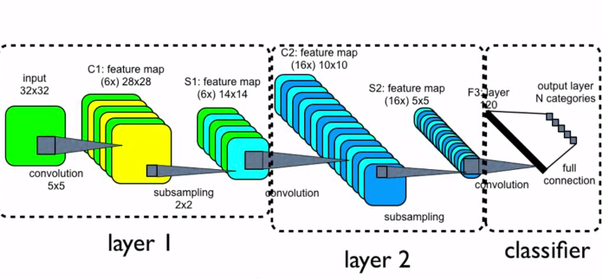
\includegraphics[width=0.7\textwidth]{img/CNN_filtre.png}
 \caption{Principe des filtres de convolution}
\end{figure}

Pour une image I de dimension (H, L, N) et un filtre F de dimension (h, l, N), on obtient une image J de dimension (H-h, L-l), la convolution est réalisée de la manière suivante :

\begin{equation}
    J(x, y) = I \star H (x, y) = \sum_{i=0}^{h - 1} \sum_{j=0}^{l- 1} \sum_{k=0}^{N - 1} I(x+i, y+j, k) \times H(i, j, k)
\end{equation}

On obtient alors une sortie de dimension (H-h, L-l, M).

Intuitivement, cette partie sert à chercher la ressemblance entre le filtre et l'image.
On devrait avoir J(x,y) < 0 si la partie de l'image I en (x,y) est très différente du filtre appliqué, et J(x,y) > 0 sinon, avec un score plus ou moins élevé selon la ressemblance.


On applique ensuite la couche d'activation. On utilise une fonction non-linéaire comme dans le cas du perceptron. 
Généralement, la fonction utilisée pour les couches de convolution intermédiaires est la fonction reLU :

$$
reLU(x) = \left\{
    \begin{array}{ll}
        x & \mbox{si } x > 0 \\
        0 & \mbox{sinon}
    \end{array}
\right.
$$

\newpage 

Cette fonction sert à ramener le résultat dans les réels positifs pour éviter une divergence au niveau des calculs, et pour augmenter l'écart relatif entre un bon score et un mauvais score : un score de 0 et en score de -1 obtenu lors de la convolution sont alors considéré comme tout aussi mauvais.

Enfin, on applique une couche de pooling, qui sert à réduire le nombre de données obtenues en sortie des 2 couches précédentes.
Le pooling cherche à "résumer" les scores d'une partie de l'image, en donnant un score qui dépend des pixels de cette partie.
Il existe plusieurs méthode de pooling, comme par exemple le pooling par moyenne ou le pooling par maximum. C'est ce dernier qui est le plus utilisé en pratique :
pour une image J, on choisi un paramètre ``stride'' S (S < L, H) et on prend la sortie K telle que :

\begin{equation}
    K(x, y) = max_{i,j \in [0, S-1] ^2 } { J(x \times S + i , y \times S + j ) }
\end{equation}


On enchaîne ainsi les couches de convolution jusqu'à une couche finale, qui sera reliée à un réseau complètement connecté (qui n'est rien d'autre qu'un simple perceptron).
Les poids à optimiser sont alors les poids des matrices qui définissent les filtres et les poids de la couche entièrement connectée.
Dans le principe, un CNN est comme un perceptron (à part pour la couche de pooling, on pourrait construire un CNN avec un perceptron), à l'exception que seulement certains poids sont liés lors de l'apprentissage.

\subsection{Application pratique}

Afin de mieux comprendre le principe du CNN, nous avons réalisé un exemple simple mais clair : on cherche à reconnaître le motif d'une croix.
Pour cela, on prend les filtres $f_1$ (diagonale gauche), $f_2$ (diagonale droite) et $f_3$ (croix centrale).
Alors en appliquant la convolution, l'activation reLU et un stride à S = 2, on obtient le résultat suivant (figure \ref{fig:convolution_filtre}) :

\begin{figure}[h]
    \center
    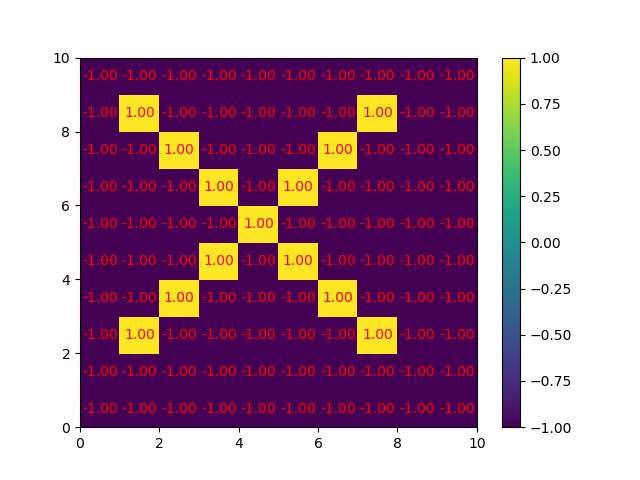
\includegraphics[width=0.5\textwidth]{img/cnn_exemple/cross/image_croix.png}
    \caption{Image à détecter}
\end{figure}

\begin{figure}[h]
    \minipage{0.32\textwidth}
        \includegraphics[width=\textwidth]{img/cnn_exemple/cross/filtre_1.png}
        \center
        (a) Filtre 1
    \endminipage\hfill
    \minipage{0.32\textwidth}
        \includegraphics[width=\textwidth]{img/cnn_exemple/cross/filtre_2.png}
        \center
        (b) Filtre 2
    \endminipage\hfill
    \minipage{0.32\textwidth}%
        \includegraphics[width=\textwidth]{img/cnn_exemple/cross/filtre_3.png}
        \center
        (c) Filtre 3
    \endminipage
    \caption{Choix des filtres pour la convolution}
\end{figure}


\newpage

\begin{figure}[h]
    \minipage{0.32\textwidth}
        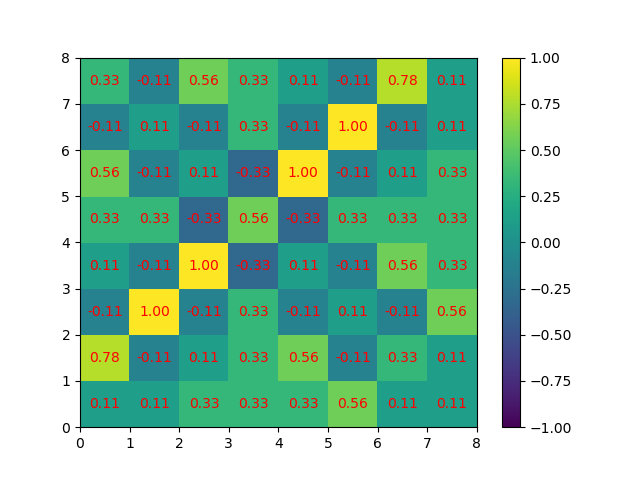
\includegraphics[width=\textwidth]{img/cnn_exemple/cross/convolution_filtre_1.png}
        \center
        (a) Convolution par le filtre 1
    \endminipage\hfill
    \minipage{0.32\textwidth}
        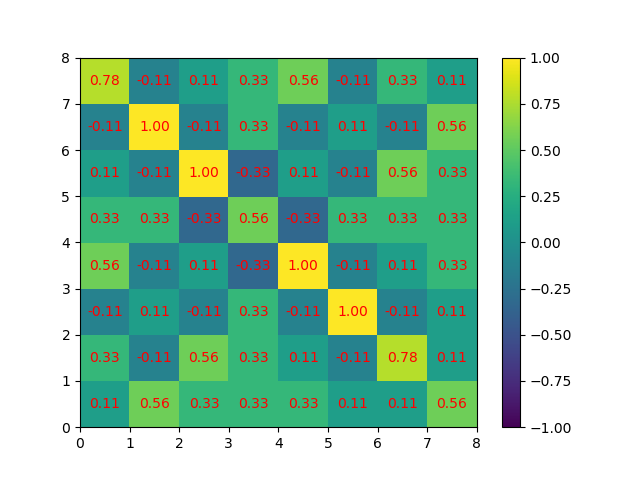
\includegraphics[width=\textwidth]{img/cnn_exemple/cross/convolution_filtre_2.png}
        \center
        (b) Convolution par le filtre 2
    \endminipage\hfill
    \minipage{0.32\textwidth}%
        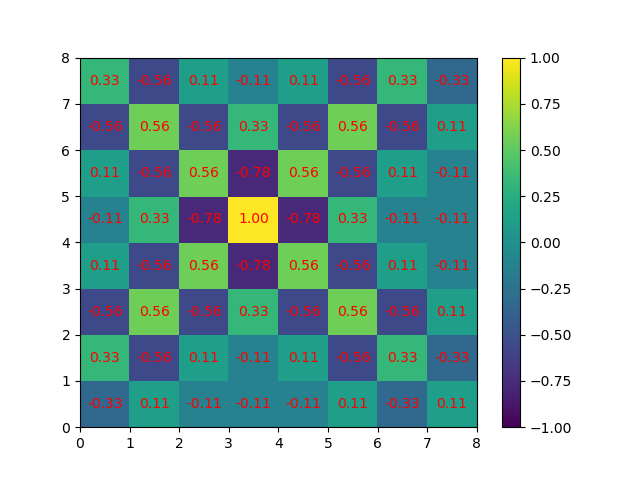
\includegraphics[width=\textwidth]{img/cnn_exemple/cross/convolution_filtre_3.png}
        \center
        (c) Convolution par le filtre 3
    \endminipage
    \center 
    \caption{Résultats de la convolution de l'image par les différents filtres}
    \label{fig:convolution_filtre}
\end{figure}

On remarque que les filtres en question réalisent bien l'action voulue : pour la première convolution, les positions des 
diagonales gauches sont mises en valeur, pour la seconde convolution, les diagonales droites sont mises en valeurs, 
et pour la troisième convolution, la croix centrale est mise en valeur. On obtient ainsi 3 channels.
\begin{figure}[h]
    \minipage{0.32\textwidth}
        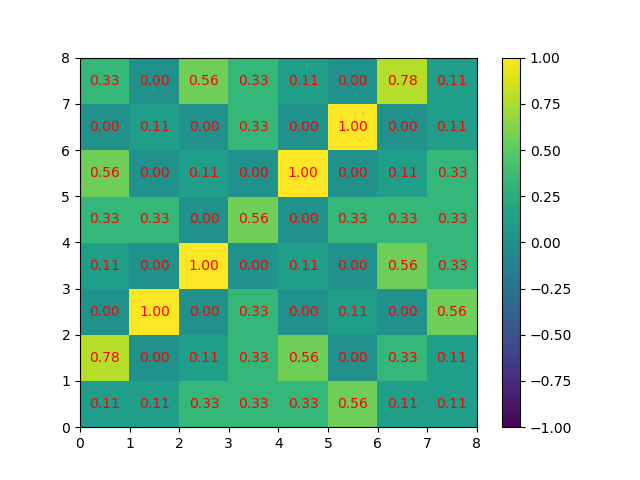
\includegraphics[width=\textwidth]{img/cnn_exemple/cross/activation_relu_1.png}
        \center
        (a) Activation reLU pour le channel 1
    \endminipage\hfill
    \minipage{0.32\textwidth}
        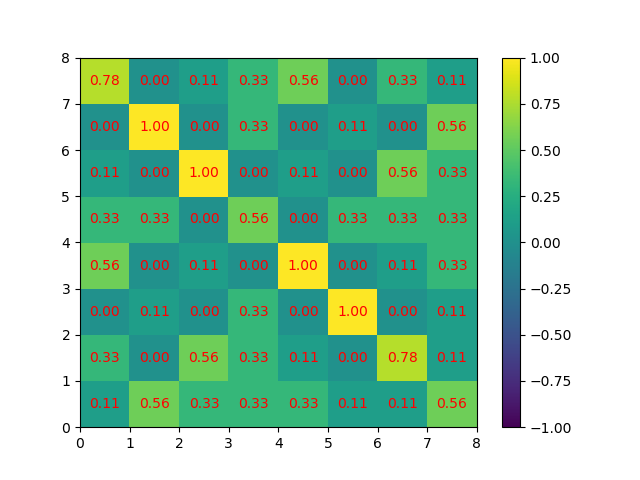
\includegraphics[width=\textwidth]{img/cnn_exemple/cross/activation_relu_2.png}
        \center
        (b) Activation reLU pour le channel 2
    \endminipage\hfill
    \minipage{0.32\textwidth}%
        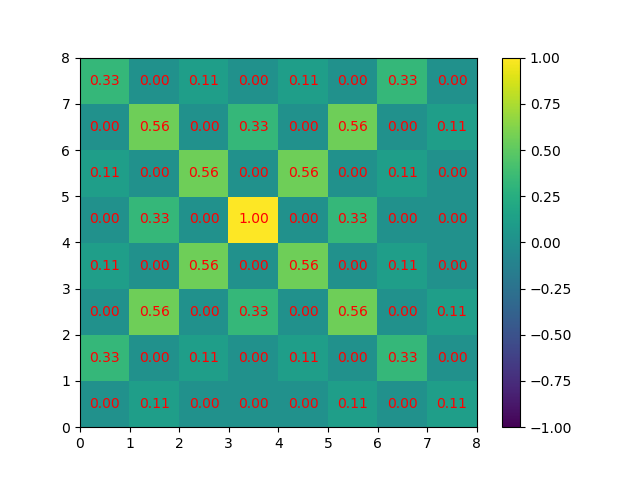
\includegraphics[width=\textwidth]{img/cnn_exemple/cross/activation_relu_3.png}
        \center
        (c) Activation reLU pour le channel 3
    \endminipage 
    \caption{Activation par la fonction reLU des différents channels.}
\end{figure}

Après l'activation, on remarque peu de changement quand aux positions des motifs recherchés : 
ces positions sont toujours bien présentes, tandis dans que le reste de l'image où les motifs ne se trouvent pas, 
les valeurs sont "mises à niveau" pour bien insister sur le fait qu'elles n'apporteront pas d'informations pertinentes 
lors du traitement par perceptron.
On applique ensuite une étape de pooling.

\newpage

\begin{figure}[h]
    \minipage{0.32\textwidth}
        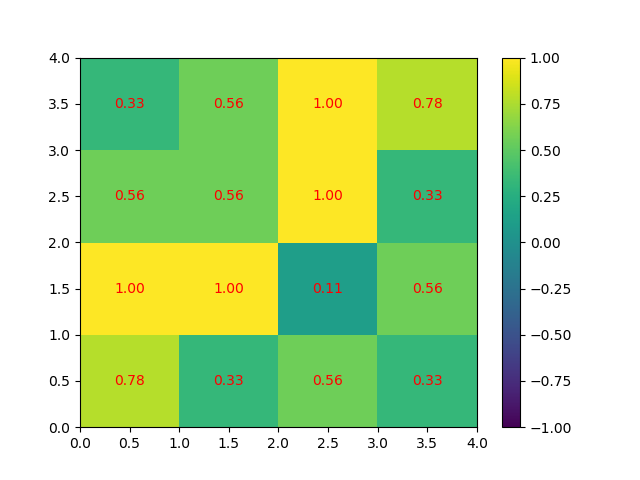
\includegraphics[width=\textwidth]{img/cnn_exemple/cross/stride_1_max.png}
        \center 
        (a) Pooling du channel 1
    \endminipage\hfill
    \minipage{0.32\textwidth}
        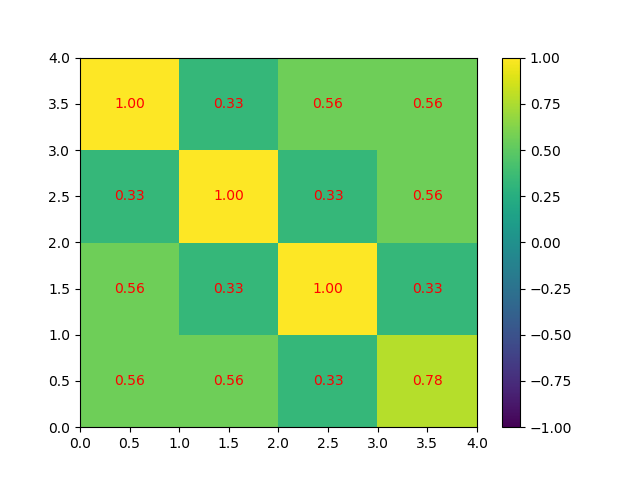
\includegraphics[width=\textwidth]{img/cnn_exemple/cross/stride_2_max.png}
        \center 
        (b) Pooling du channel 2
    \endminipage\hfill
    \minipage{0.32\textwidth}%
        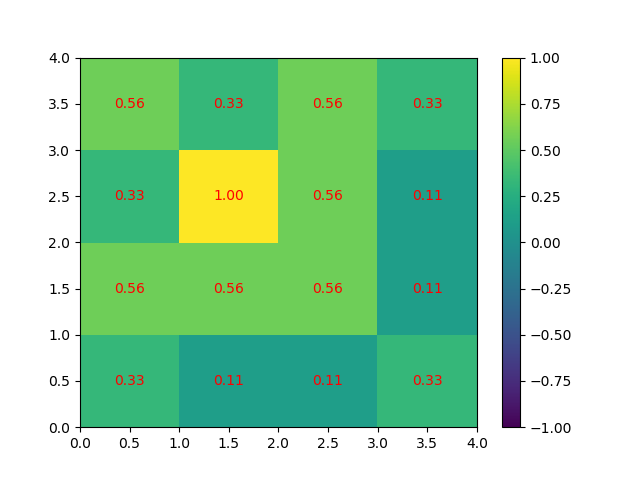
\includegraphics[width=\textwidth]{img/cnn_exemple/cross/stride_3_max.png}
        \center
        (c) Pooling du channel 3
    \endminipage
    \caption{Pooling max des différents channels avec S = 2}
\end{figure}

On peut ainsi réduire les dimensions de l'image, tout en conservant une position globale des caractéristiques intéressantes.

On aperçoit alors l'apparition de zones à scores élevés par rapport au reste.
On passe ensuite ces résultats dans un "réseau complètement connecté" (fully connected network) 
afin de pouvoir exploiter le contraste que ce réseau à convolution a mis en valeur.


Si on applique le même traitement à une autre figure (ici un carré), on remarque que le résultat est beaucoup moins contrasté :

\begin{figure}[h]
    \center
    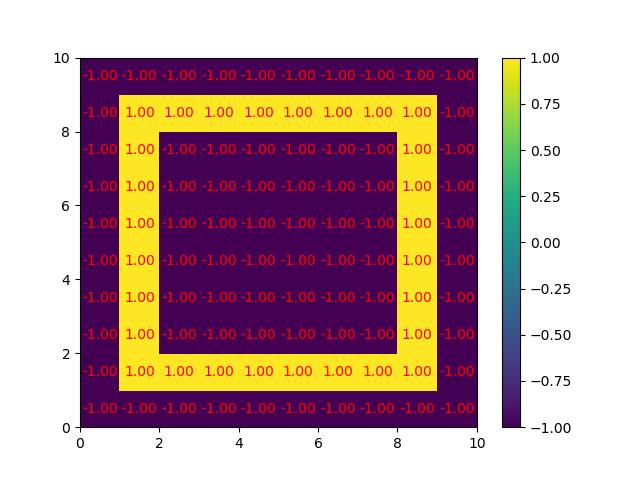
\includegraphics[width=0.5\textwidth]{img/cnn_exemple/square/image_carre.png}
    \caption{Image à éviter}
\end{figure}


\begin{figure}[!htb]
    \minipage{0.32\textwidth}
        \includegraphics[width=\textwidth]{img/cnn_exemple/square/filtre_1.png}
        \center 
        (a) Filtre 1
    \endminipage\hfill
    \minipage{0.32\textwidth}
        \includegraphics[width=\textwidth]{img/cnn_exemple/square/filtre_2.png}
        \center 
        (b) Filtre 2
    \endminipage\hfill
    \minipage{0.32\textwidth}%
        \includegraphics[width=\textwidth]{img/cnn_exemple/square/filtre_3.png}
        (c) Filtre 3
    \endminipage
    \caption{Choix des filtres pour la convolution}
\end{figure}

\newpage

\begin{figure}[h]
    \minipage{0.32\textwidth}
        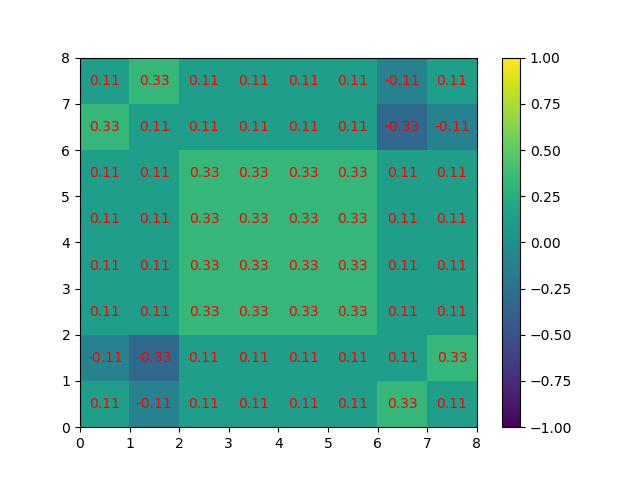
\includegraphics[width=\textwidth]{img/cnn_exemple/square/convolution_filtre_1.png}
        \center 
        (a) Convolution du carré par le filtre 1
    \endminipage\hfill
    \minipage{0.32\textwidth}
        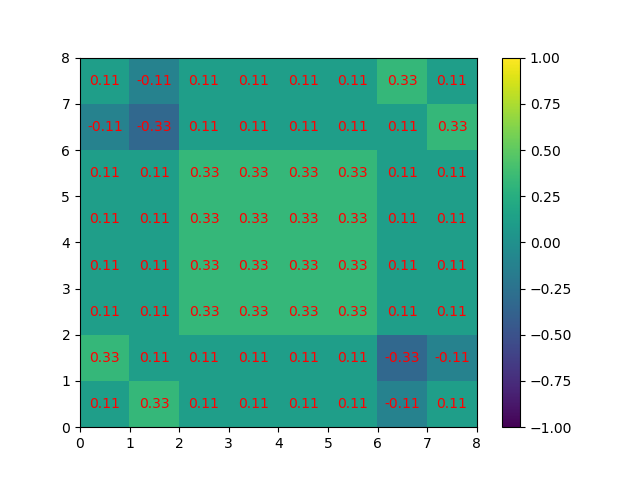
\includegraphics[width=\textwidth]{img/cnn_exemple/square/convolution_filtre_2.png}
        \center 
        (b) Convolution du carré par le filtre 2
    \endminipage\hfill
    \minipage{0.32\textwidth}%
        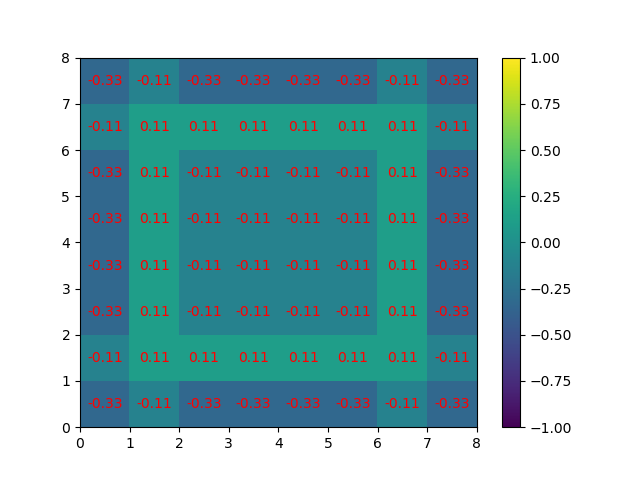
\includegraphics[width=\textwidth]{img/cnn_exemple/square/convolution_filtre_3.png}
        \center 
        (c) Convolution du carré par le filtre 
    \endminipage
    \caption{Résultats de la convolution de l'image par les différents filtres}
\end{figure}


\begin{figure}[h]
    \minipage{0.32\textwidth}
        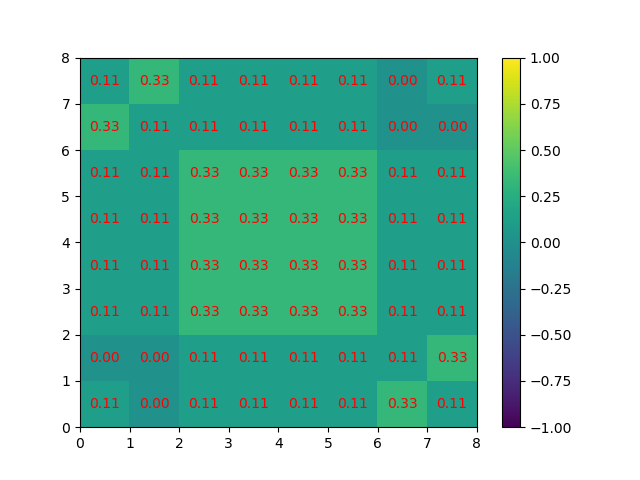
\includegraphics[width=\textwidth]{img/cnn_exemple/square/activation_relu_1.png}
        \center 
        (a) Activation reLU pour le channel 1
    \endminipage\hfill
    \minipage{0.32\textwidth}
        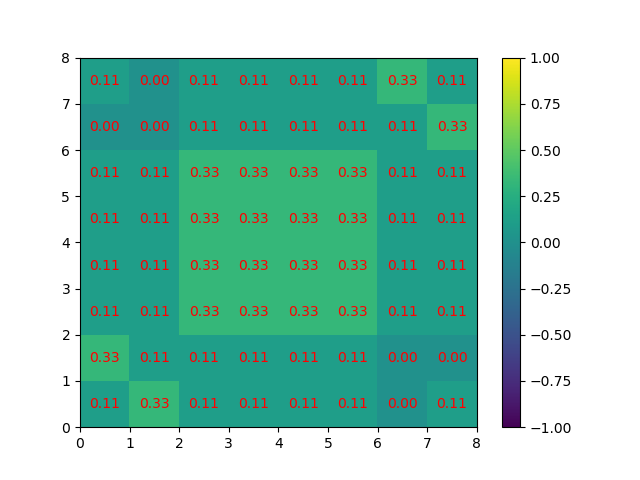
\includegraphics[width=\textwidth]{img/cnn_exemple/square/activation_relu_2.png}
        \center 
        (b) Activation reLU pour le channel 2
    \endminipage\hfill
    \minipage{0.32\textwidth}%
        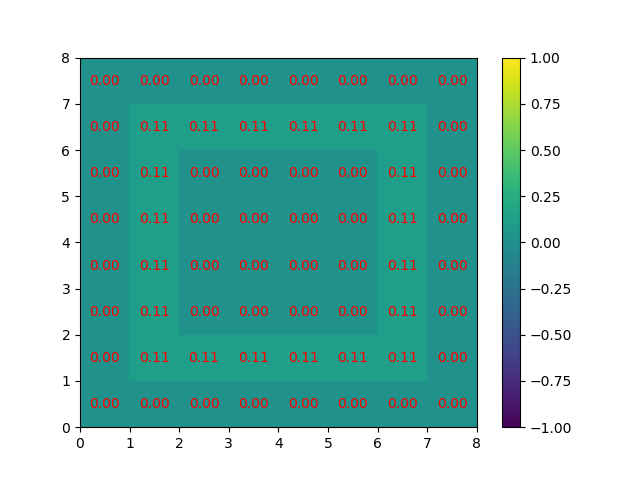
\includegraphics[width=\textwidth]{img/cnn_exemple/square/activation_relu_3.png}
        \center 
        (c) Activation reLU pour le channel 3
    \endminipage
    \caption{Activation par la fonction reLU des différents channels.}
\end{figure}

\newpage

\begin{figure}[h]
    \minipage{0.32\textwidth}
        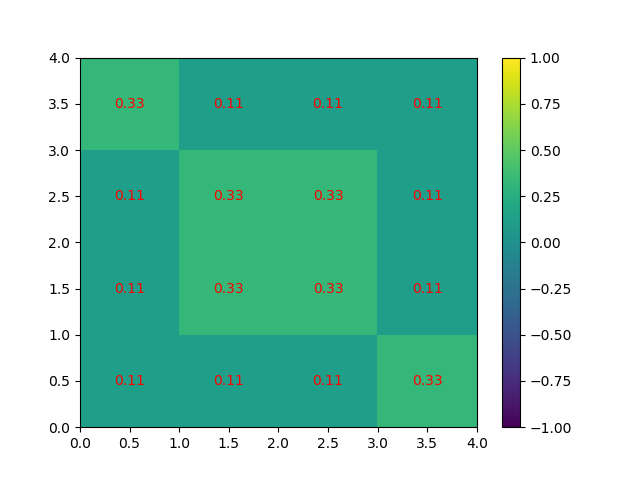
\includegraphics[width=\textwidth]{img/cnn_exemple/square/stride_1_max.png}
        \center 
        (a) Pooling du channel 1
    \endminipage\hfill
    \minipage{0.32\textwidth}
        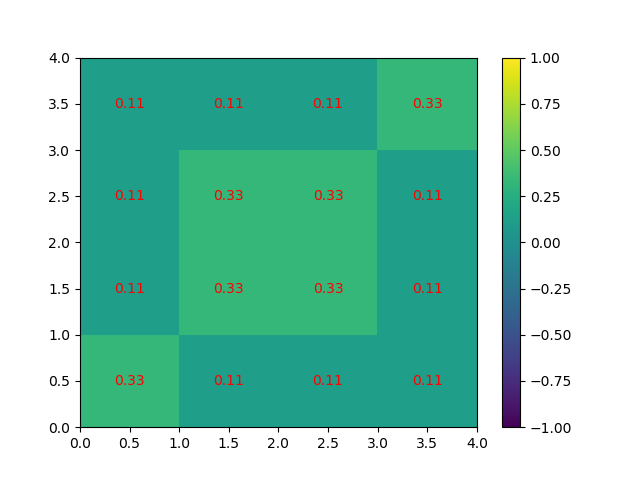
\includegraphics[width=\textwidth]{img/cnn_exemple/square/stride_2_max.png}
        \center 
        (b) Pooling du channel 2
    \endminipage\hfill
    \minipage{0.32\textwidth}%
        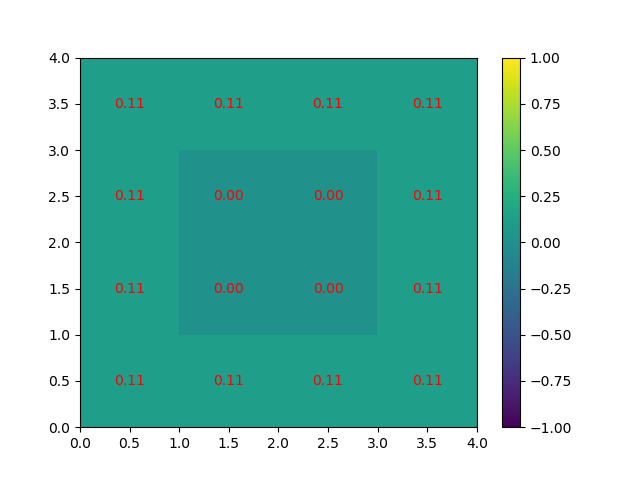
\includegraphics[width=\textwidth]{img/cnn_exemple/square/stride_3_max.png}
        \center 
        (c) Pooling du channel 3
    \endminipage
    \caption{Pooling max des différents channels avec S = 2} 
\end{figure}



On remarque que le résultat final est beaucoup plus flouté, et n'apporte pas d'informations pertinentes pour le réseau de 
neurones arrivant derrière.


Dans le cas présenté ci-dessus, nous avons choisi nous-même les paramètres des filtres appliqués pour la convolution,
en se basant sur l'intuition.
En pratique, les poids des matrices composants les filtres sont appris comme des paramètres standards d'un réseau de neurones.

\newpage

\subsection{Résultats}

Nous avons comparé les performances du CNN avec un réseau de neurones complètement connecté sur la base de données MNIST.

Les entraînements ont été réalisé sur 60000 éléments, par minibatches de 32.

Les réseaux considérés sont les suivants : 
\begin{itemize}
    \item Un perceptron de petite dimension (une couche cachée de taille 512)
    \item Un perceptron de grande dimension (deux couches cachées, de taille 4096 et 64)
    \item Un CNN (32 filtres de tailles 3$\times$3, 64 filtres de tailles 3$\times$3, un pooling max de taille 2$\times$ 2, une couche cachée de taille 128)
\end{itemize}

Le perceptron de grande dimension a été choisi de façon à avoir un nombre équivalent de paramètres avec le CNN.


\begin{figure}[h]
    \center 
    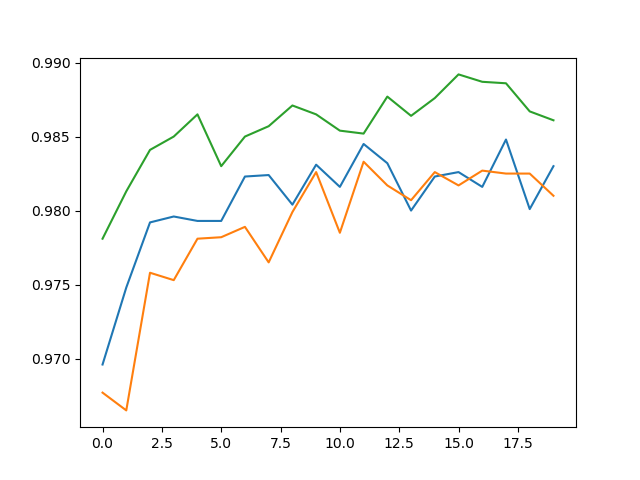
\includegraphics[width=0.6\textwidth]{img/fc_vs_cnn.png}
    \caption{Comparaisons des performances pour des perceptrons et pour un CNN en fonction du nombres d'epochs. 
    CNN en vert, perceptron de petite dimension en bleu, perceptron de grande dimension en orange}
\end{figure}

On voit qu'au bout d'un passage complet sur les données (par minibatches de 32), le CNN obtient de meilleurs résultats que les 
perceptrons. De plus, on remarque que le perceptron de grande dimension converge plus lentement que le réseau de petite dimension.
Le CNN sert alors à obtenir une convergence plus rapide (comme un perceptron de petite taille),
et obtient de meilleurs résultats à termes car il n'est pas limité par son nombre de paramètres (comme un perceptron de grande dimension).

\newpage
La taille de filtres a également une influence sur l'entraînement du CNN. En effet, les filtres ont pour but de trouver des "motifs" dans l'image et de le mettre en valeur par rapport au reste de l'image. Plus le motif est petit, plus il sera facile d'entraîner le filtre, mais le motif alors trouvé ne sera pas forcement pertinent pour la classification. Inversement, plus le filtre est de grande dimension, plus il pourra rechercher des motifs complexes, mais la convergence sera alors plus compliquée et pas aussi stable.


\begin{figure}[h]
    \center 
    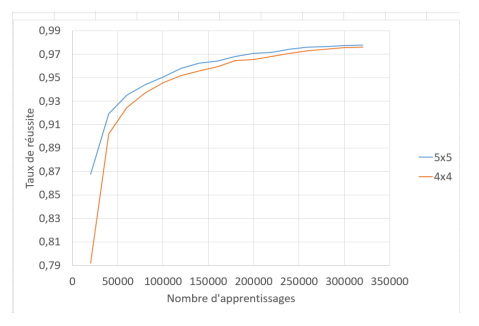
\includegraphics[width=0.6\textwidth]{img/comparaison_filtres.png}
    \caption{Comparaison des performances pour des perceptrons et pour un CNN en fonction du nombres d'epochs}
\end{figure}

En observant les résultats, on remarque que les filtres de 5$\times$5 ont un bon rapport performance/vitesse de convergence.


\subsection{Utilisation de TensorFlow}

TensorFlow a été utilisé pour coder le CNN. Un codage à la main du CNN aurait été possible et très instructive mais complexe et chronophage. L'utilisation de TensorFlow a permis d'avancer plus rapidement sur la programmation du CNN. Par ailleurs, le fonctionnement de chaque bloc utilisé par TensorFlow pour coder un CNN avait été vu en détail précédemment, ce qui a permis de comprendre ce qui se cachait derrière les fonctions de haut niveau proposées par TensorFlow.

TensorFlow est facile d'installation sous Linux et sa prise en main est plutôt aisée. Il existe de nombreux tutoriels pour construire des CNN. Cependant, le développement de TensorFlow évolue rapidement et la documentation n'est pas forcément très complète. L'implémentation de fonctionnalités précises est donc parfois difficile. Il est nécessaire de faire de longues recherches pour trouver les fonctions désirées.

Cependant, en plus de réduire grandement le temps nécessaire pour programmer un CNN efficace, TensorFlow offre une interface graphique (figure \ref{fig:interface_TF}) très utile pour suivre en direct la convergence du CNN. On peut ainsi détecter rapidement le mauvais paramétrage du CNN et le modifier sans attendre d'avoir mis à jour le CNN sur les $n$ batches prévus à l'avance.

\begin{figure}[h]
 \centering
 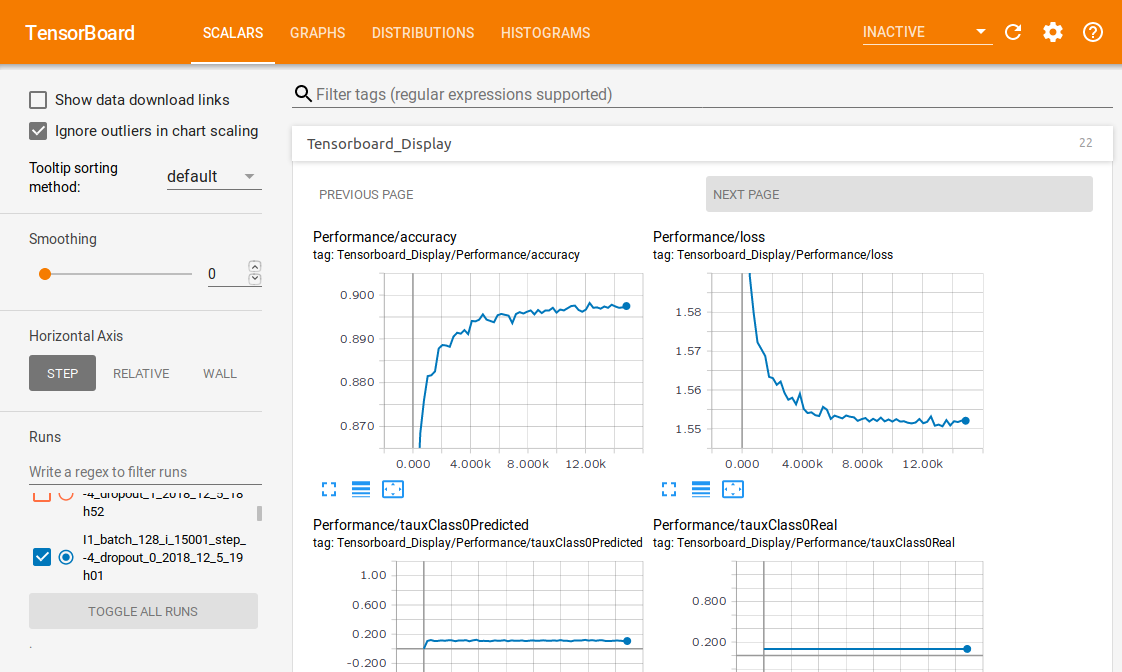
\includegraphics[width=0.7\textwidth]{img/interface_TF.png}
 \caption{TensorBoard avec visualisation en direct des performances du réseau de neurones}
 \label{fig:interface_TF}
\end{figure}


L'exploitation des résultats a posteriori s'avère plus compliquée. L'interface de TensorFlow offrant des fonctionnalités plutôt limitées, l'utilisation d'un post-traitement est indispensable. Il est par exemple impossible de réaliser des moyennes sur plusieurs runs. Après quelques recherches, nous avons réussi a extraire le taux de réussite en fonction du nombre d'apprentissages à partir des données brutes générées par TensorFlow. L'extraction du taux de réussite en fonction du temps de calcul s'est avérée plus compliquée. Nous remercions Julien \textsc{Gérard} qui nous a beaucoup aidé sur ce point. Il nous a en effet indiqué avoir trouvé dans le code source de TensorFlow la fonction $wall\_time$ qui permet d'extraire le temps écoulé depuis le lancement des calculs pour chaque relevé du taux de réussite.

Nous avons testé TensorFlow avec un CNN pour MNIST. Grâce au post-traitement, nous avons pu tracer une moyenne du taux de réussite en fonction du nombre d'apprentissages réalisées (figure \ref{fig:tb_post_traitement}).

\begin{figure}[h]
 \centering
 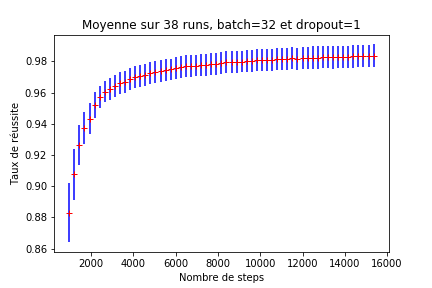
\includegraphics[width=0.7\textwidth]{img/tb_post_traitement.png}
 \caption{Taux de réussite en fonction du nombre d'apprentissages pour notre CNN sous TensorFlow}
 \label{fig:tb_post_traitement}
\end{figure}

Le post-traitement pourraient être utilisé pour déterminer les effets de la taille des batchs ou encore du dropout. Se pose alors la question de la nature de l’abscisse. Est-il préférable de d'utiliser le nombre d'apprentissages ou le temps ?
Nous avons choisi de ne pas traiter en profondeur ces questions pour nous concentrer sur le c\oe ur de notre sujet, le Q Learning. Cette question reste cependant une piste qui pourrait être explorée dans un futur projet.
